\section{Semantic rules}

\subsection{EPNs}

 \begin{enumerate}
   \item All \glyph{state variables} associated with a Stateful Entity Pool Node should be unique and not duplicated within that node.
   \item If a state variable is used in one EPN then is must be used in all equivalent stateful EPNs\footnote{A stateful EPN is equivalent if the EPNs are identical when their state descriptions are ignored.}.
   \item EPNs should not be orphaned (i.e.\, they should be associated with at least one arc).
 \end{enumerate}

\subsection{Process Nodes}

As described in \sect{process}, the \glyph{consumption} and \glyph{production} arcs converge before connecting to the process node (\fig{process-sidedness}). This defines the EPNs that are the input and outputs of an irreversible process. Since, processes can be reversible in the following rules we refer to these groupings as the ``left-hand-side'' (LHS) and ``right-hand-side'' (RHS) of the process\footnote{Note this designation is purely for grouping and is used even then the sides of the reaction are above and below the process.}. For convenience we will also collectively refer to the \glyph{consumption} and \glyph{production} arcs as \emph{flux} arcs.

\begin{figure}[H]
  \centering
  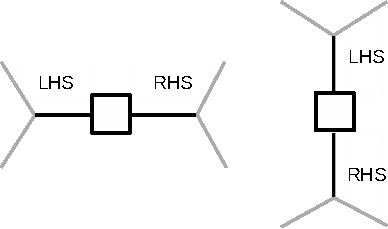
\includegraphics[scale = 0.8]{images/build/process_sidedness.pdf}
  \caption{An illustration of the ``sidedness'' of a process. The designation of LHS and RHS is essentially arbitrary.}
  \label{fig:process-sidedness}
\end{figure}

\subsubsection{Flux Arcs}

\begin{enumerate}
\item All process nodes (with the exception of \glyph{phenotype}) must have a LHS and RHS.
    \item All EPNs on the LHS of a process must be unique.
    \item All EPNs on the RHS of a process must be unique.
    \item All \glyph{phenotype} glyphs must be associated with at least one modulation arc.
    \item The EPNs that make up the LHS of the process should be consistent with the RHS, i.e., the process should constitute a    balanced biochemical reaction.
    \item Once the stoichiometry of a flux arc is displayed in a map then all other flux arcs should
    display their stoichiometry make.
    \item If the stoichiometry is undefined or unknown this should be indicated by the use of a question mark (``?''). 
   \item If more than one set of stoichiometries can be applied to the flux arcs of the process then the stoichiometry of the flux arcs must be displayed.
\end{enumerate}  

\subsubsection{\glyph{Association}}

  \begin{enumerate}
    \item An \glyph{Association} is always an irreversible process.
    \item If a \glyph{Complex} is on the RHS of the association then
  there must be at least 2 EPNS on the LHS.
\end{enumerate}  

\subsubsection{\glyph{Dissociation}}
  \begin{enumerate}
    \item A \glyph{Dissociation} is always an irreversible process.
    \item If a \glyph{Complex} is on the LHS of the dissociation then there must be at least 2 EPNs on the RHS.
\end{enumerate}  

\subsubsection{Modulation}
\label{sec:mod-semantics}

As discussed in \sect{concepts}, it is implied, but not defined explicitly that the process has a rate at
which it converts its LHS EPNs to its RHS EPNs (and vice-versa in the case of a reversible process). This concept is
important in understanding how the \PDl describes process modulation.

\begin{enumerate}
\item A \glyph{process} with no modulations has an underlying ``basal rate''
  which describes the rate at which it converts inputs to outputs.
\item A \glyph{modulation} changes the basal rate in an unspecified fashion.
\item A \glyph{stimulation} is a modulation that increases the basal rate.
\item An \glyph{inhibition} is a modulation that decreases the basal rate.
\item The above types of modulation, when assigned to the same process, are combined and have a multiplicative effect on the basal rate of the process.
\item Modulators that do not interact with each other in the above manner, should be drawn as modulating different process nodes. Their effect is therefore additive.
\item At most one \glyph{necessary stimulation} can be assigned to a process node. Two \glyph{necessary stimulations}
  would imply an implicit AND or OR operator. For clarity only
  one \glyph{necessary stimulation} can be assigned to a \glyph{process}, and such combinations must be
  explicitly expressed using \glyph{logical operators}. 
\item At most one \glyph{catalysis} can be assigned to a
  \glyph{process}. Modulation by a catalysis arc implies that the exact biochemical mechanism underlying
  the process is known. In this context two \glyph{catalysis} cannot
  be assigned to the same process node as they represent
  independent reactions. Other EPNs can be assigned to the same process as a catalysis, such as modulators, stimulators, and
  inhibitors, and will have a multiplicative modulation on the reaction rate defined by the catalysis.
\end{enumerate}

\subsubsection{Reversible Processes}
\label{sec: semantics reversible procs}

A process is deemed to be reversible if it has \glyph{production} arcs on both the LHS and RHS of a process node \fig{process-reversibility}. Semantically, the \glyph{production} arc can be thought of as allowing a reversible flow of entities between the \glyph{process} and the \glyph{EPN}. A \glyph{consumption} arc only permits an irreversible flow from the \glyph{EPN} to the \glyph{process}. In this way, the \glyph{consumption} arc forces the \glyph{process} to be irreversible. \glyph{Consumption} arcs cannot be associated with both sides of a \glyph{process} as this would prohibit any flow through the \glyph{process}.

\begin{figure}[H]
  \centering
  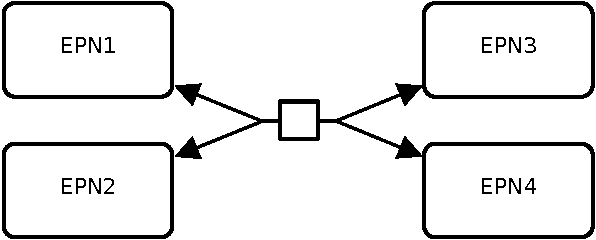
\includegraphics[scale = 0.8]{images/build/reversible_process.pdf}
  \caption{A valid reversible process. A process is reversible if its LHS and RHS contain only \glyph{production} arcs.}
  \label{fig:process-reversibility}
\end{figure}
 
\begin{enumerate}
\item  A mixture of \glyph{consumption} and \glyph{production} arcs on the same side of a \glyph{process} is not permitted.

\item The semantics of \glyph{modulation} is the same as for irreversible processes, .i.e., the amount of entity in the modulation pool affects the rate of the process.
\end{enumerate}

 
\subsection{Cloning}

SBGN allows identical nodes to be duplicated on a map if they are
explicitly marked as such. This is done using a \glyph{clone marker}. The details are shown in table \ref{tab:processduprules}.


\begin{center}
\tablecaption{Duplication rules.}
\label{tab:processduprules}
\begin{footnotesize}
\tablefirsthead{\hline
  Node & Can be duplicated & Indication & Additional Rules\\\hline}
\tablehead{\hline
\multicolumn{4}{|l|}{\small\sl continued from previous page}\\
\hline\hline
  Node & Duplicate? & Indication & Additional Rules\\\hline\hline}
\tabletail{\hline
\multicolumn{4}{|r|}{\small\sl continued on next page}\\
\hline}
\tablelasttail{\hline}
\begin{supertabular}{|l|c|p{4cm}|p{3.5cm}|}\hline
Compartment   & N & & \\\hline
SimpleChemical & Y & \glyph{Simple clone marker} & \\\hline
UnspecifiedEntity & Y & \glyph{Simple clone marker} & \\\hline
EmptySet & Y & & \\\hline
Perturbing Agent & Y & \glyph{Simple clone marker} & \\\hline
Phenotype & Y & \glyph{Simple clone marker} & \\\hline
MultimerChemicalEntity & Y & \glyph{Simple clone marker} & \\\hline
StatefulEntityPool & Y & \glyph{Labeled clone marker} & \\\hline
Macromolecule & Y & \glyph{Labeled clone marker} & \\\hline
MultimerMacromolecule & Y & \glyph{Labeled clone marker} & \\\hline
Nucleic\-Acid\-Feature & Y & \glyph{Labeled clone marker} & \\\hline
Complex & Y & \glyph{Labeled clone marker} & \\\hline
Process & Y & None & \\\hline
OmittedProcess & Y & As Process  & \\\hline
UncertainProcess & Y & As Process  & \\\hline
Association & Y & As Process  & \\\hline
Dissociation & Y & As Process  & \\\hline
LogicalOperator & Y & None & \\\hline
AND & Y & None & \\\hline
OR & Y & None & \\\hline
NOT & Y & None & \\\hline
Equivalence & Y & None & \\\hline
\end{supertabular}
\end{footnotesize}
\end{center}


\subsection{Compartment spanning}

An \glyph{EPN} cannot \emph{belong} to more than one
\glyph{compartment}. However, an EPN can be \emph{drawn} over more than one
\glyph{compartment}. In such cases, the decision on which is the owning
\glyph{compartment} is deferred to the drawing tool or the
author. A \glyph{complex} may contain EPNs which belong to different
\glyph{compartments} and in this way a \glyph{complex} can be used to describe
entities that span more than one {compartment}.

This restriction makes it impossible to represent in a semantically
correct way a macromolecule that spans more then one compartment ---
for example a receptor protein. It is clearly desirable to be able to
show a macromolecule in a manner that the biologist expects (i.e.,
spanning from the outside through the membrane to the
inside). Therefore, the author is recommended to draw the
macromolecule across compartment boundaries, but the underlying SBGN
semantic model will assign it to only one.

Note that this has implications for auto-layout algorithms as
they will only be able to treat such \glyph{entity pool nodes} as contained within
a \glyph{compartment} and will have no way of knowing a macromolecule spans a
compartment.

The current solution is consistent with other Systems Biology
representations such as SBML and BioPAX. For more information about the
problems representing membrane spanning proteins and the rationale
behind the current solution see \sect{postponed}.

\subsection{Submaps}

The submap is a visual device that allows the detail of an \PD map to be exported into another \PD map and replaced by a \glyph{submap} glyph, which acts as a place-holder. This is described and illustrated in \sect{submap}. In the following discussion we will refer to the original map as the \emph{main} map and the map containing the export detail as the submap. 

\begin{enumerate}
\item For a valid mapping between an EPN in the map and submap to exist the identifiers in the \glyph{tag} and the submap terminal must be identical and their associated entity pool nodes must be identical.
\item If the same EPN is present in the map and a submap, then they must be mapped to each other.
\item Since the main map and submap share the same namespace, an EPN that is cloned in the main map must also be
marked as cloned in the submap --- even if there is only one copy of the EPN in the submap. The converse applies when the EPN in the submap is cloned\footnote{This has the additional benefit of ensuring that main maps and submaps do not need to be modified if the submap is exanded and collapsed by a viewing or editing tool.}.
\end{enumerate}

\subsection{Equivalence operator}
\label{sec:eq-semantics}

\begin{enumerate}
    \item Pools should not overlap
    \item A \glyph{process} should not affect \glyph{EPNs} belonging or deriving from both sides of an \glyph{equivalence operator}
    \item For \glyph{simple chemicals} (stateless \glyph{EPNs}) it is not allowed to show specifics both as input and as output of a pathway
\end{enumerate}

For automatic verification, the first rule can be transformed into the following validation rules:
\begin{enumerate}[label=(\alph*)]
    \item Split generic processes and influences into specific ones.
    \item There should not be any repeating processes or influences after this splitting procedure is complete.
\end{enumerate}
